\documentclass{mcmthesis}
\mcmsetup{CTeX = false, 
        tcn =57566, problem = B,
        sheet = true, titleinsheet = true, keywordsinsheet = true,
        titlepage = false, abstract = true}
\usepackage{palatino}
\usepackage{array}
\bibliographystyle{apalike}
\title{An optimized design of the area following the toll barrier }

\begin{document}

	
	
\begin{abstract}
	
In order to determine the optimal shape and the size of the toll plaza, this paper proposes a simulation model for New Jersey Turnpike Authority to ameliorate the performance of the toll station.

First, after referencing to the common designs of toll stations in current use and analyzing the differences, the plaza is simulated by a number of tollbooths of different types. Each tollbooth is configurable in the simulation for vehicle passage type, charging mode and lane direction which will direct the vehicles into the merging flow. The performance is evaluated by a weighted average of throughput index, accident rate index and cost index. The weights are determined by principal component analysis. 

The vehicles are simulated by a set of rectangles in a two-dimensional plane, with a moving strategy written based on car following (CF) model \footnote{Reuschel and Pipes in 1956, Herman and Rothory in 1960}, GM model \footnote{Gazis,Herman and Rothery} and Nagel-Schreckenberg (NS) model \footnote{K.Nagel and M.Schreckenberg in 1992}. The vehicles are generated by the tollbooth by a probabilist model, given a fixed traffic flow and then fired for the merge. The vehicles submit to possible collisions with other vehicles and the road boundary. Both autonomous cars and human-driven cars are simulated, equipped with adapted moving strategies.

With this generalized and adapted model, the throughput can be obtained on calculating the average throughput result of multiple simulations. The accident rate is obtained by a larger set of simplified simulations. The cost is calculated by the construction area and tollbooth number. The experiments on $MATLAB$ with different parameters of tollbooth and shape give an analysis of several design schemes, detailed in the report.

In the last part, with different parameters set, an improved design in terms of throughput is proposed on running an optimization algorithm. Various proportions of autonomous vehicles and tollbooths are also tested.


\begin{keywords}
;
\end{keywords}
\end{abstract}

\maketitle
\tableofcontents
\clearpage








\section{A letter to the New Jersey Turnpike Authority}


New Jersey Turnpike Authority,

Our team has proposed an optimized toll station design allowing the increase of throughput and the decrease of cost and accident rate. And a new mathematical model is built in order to help evaluate the performances of designs. 

More specifically, the performance model is developed after taking all important elements related to this problem into consideration, like number of lanes and tollbooths, proportions of tollbooths, varieties of vehicles, change of flows, every decision made by drivers to turn right or left and traffic conditions. 



\section{Introduction}

\subsection{Statement of the problem}


  The design of toll station is undoubtedly a kind of art as it is hard to find a balance among safety, capacity and cost facing different situations. But it also acts as an essential part in the high-way traffic system. As a promotion of toll station is in demand, we apply mathematical methods and function models for optimize our design, striving to increase the throughput, decrease the cost and accident rate.



\begin{itemize}

\item 
\end{itemize}







\begin{Theorem} \label{thm:latex}

\end{Theorem}

\begin{Lemma} \label{thm:tex}

\end{Lemma}

\begin{proof}
The proof of theorem.
\end{proof}

\subsection{Assumptions}

\begin{itemize}
	\item All the vehicles leave the tollbooths with a given speed.
	\item There is a critical flow $F_c$, when the total flow  $F_t>F_c$, the vehicles begin to queue up before the toll station.
	\item The proportions of different types of vehicles are invariable along the time.
	\item In light traffic, the tollbooths the vehicles arrive are random.
	\item We take each vehicle as a point located on the center of gravity, but the vehicles still have the volume.
    \item Time is devided into 1 second, drivers' decisions in every second depend on the surroundings and the status are updated every second. \footnote{Nagel-Schreckenberg model applied.}
	\item The accelerations of all the vehicles depend on the others who surround themselves.\footnote{Car following model applied.}
	\item The biggest wheel steering angle is $45^{\circ}$, and the turning radius is negleted.
\end{itemize}



Here we list the elements that will influence the throughput of our toll station:

\begin{tabular}{|m{7cm}<{\centering}|p{7cm}<{\centering}|}
	\hline
	Notations & Meanings \\
	\hline
	 $L$ &  Number of lanes \\
	\hline
	 $B$ &  Number of tollbooths\\
	 \hline
     $F_t$ & 	 Total flow\\
     \hline
     $F_c$ & Critical flow (the maximum of the total flow)\\
     \hline
     $P_l$,  $P_m$, $P_s$ & Probability of large-scale automobiles, midium-sized vehicles and compact cars\\
     \hline
     $v_{this}$, $a_{this}$ & Speed and acceleration of the vehicle we study\\
     \hline
      $v_n$, $a_n$ &  Speed and acceleration of the other vehicles which surround the vehicle we study\\
   \hline
     
\end{tabular}


\section{Analysis of the Problem}
\begin{figure}[htbp]
\small
\centering
\caption{Toll station \cite{note}} \label{fig:Ts}
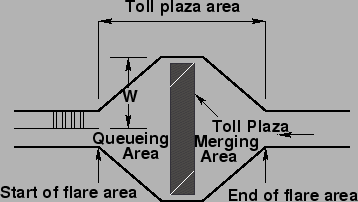
\includegraphics{img3.png}
\end{figure}

Due to the discrete traffic problem we meet, here we try to apply some mathematical models, and we take Nagel-Schreckenberg (NS) model \cite{acelluar}, CF (car following) model and GM model for reference.

In our merging area, all the vehicles from $B$ tollbooths are merging into $L$ lanes. To begin with, every fifteen minutes there is $F_t$ through the tollbooths, the flows of large-scale automobiles, midium-sized vehicles and compact cars are $F_tP_l$, $F_tP_m$, $F_tP_s$.

Now we focus on one vehicle, the speeds of the other vehicles around it are taken as vector quantities which will be added on the one chosen.  The relative speeds and relative distances of those vehicles around in last second will influence the decision the vehicle chosen takes in the next second. 

Based on the active vehicles on the road and the road shape, the driver's decision includes acceleration on each direction \footnote{considering safe distance and GM model applied.}.


The total acceleration is constitutedy of 3 parts: 
$$\overrightarrow{a_{this}(t)}=\overrightarrow{a_i(t)}+\overrightarrow{a_r(t)}+\overrightarrow{a_a(t)}$$

In which case (this $\ne$ $n$),
$$\overrightarrow{a_i(t)}=\overrightarrow{a_{interaction}(t)}=\lambda (v_{this}(t))^m \times \sum_n\frac{v_n(t)-v_{this}(t)}{(d_n(t))^l}\times \overrightarrow{dir_{n,this}(t)}$$
$$d_n(t)=distance_n(t)=\sqrt{\delta pos_x(t)^2+\delta pos_y(t)^2}$$
$$\overrightarrow{dir_n(t)}=\frac{(pos_x-pos_{x,n},pos_y-pos_{y,n})}{\parallel (pos_{x,this}-pos_{x,n},pos_{y,this}-pos_{y,n}) \parallel} $$\\
$$\overrightarrow{a_r(t)}=\overrightarrow{a_{road}(t)}=\alpha \times distance_{baundary-left}^{-l'} \times v(t)^m'\times \overrightarrow{right} \times 1_{d<d_{critical}$$
	$$+\alpha \times distance_{baundary-right}^{-l'} \times v(t)^m'\times \overrightarrow{left} \times 1_{d<d_{critical}}$$
$$distance_{baundary}=\arrowvert pos_x-pos_{distance}(pos_y)} \arrowvert$$\\
$$a_a(t)=a_{acceleration}(t)=\beta (v_{max}-v(t)) \times a_{max} \times \overrightarrow{forward}$$\\
Here $\lambda$, $l$,$m$, $\alpha$, $l'$, $m'$, $\beta$ and $a_{max}$ are the parameters that we can adjust.

Our simulation comes as follows:















\section{The Model Results}


\section{Validating the Model}


\section{Conclusions}

\section{A Summary}


\section{Evaluate of the Mode}

\section{Strengths and weaknesses}


\subsection{Strengths}
\begin{itemize}
\item \textbf{Applies widely}\\

\item \textbf{Improve the quality of the airport service}\\

\item \textbf{}\\
\end{itemize}


\begin{appendices}

\section{First appendix}


Here are simulation programmes we used in our model as follow.\\

\textbf{\textcolor[rgb]{0.98,0.00,0.00}{Input matlab source:}}
\lstinputlisting[language=Matlab]{./code/matlab1.m}

\section{Second appendix}

some more text \textcolor[rgb]{0.98,0.00,0.00}{\textbf{Input C++ source:}}
\lstinputlisting[language=C++]{./code/sudoku.cpp}

\end{appendices}

	\nocite{*}

\bibliography{math}

	
\end{document}

